\documentclass[a4paper,12pt]{scrartcl}
\usepackage{nameref}
\usepackage[hyphens]{url}
\usepackage{hyperref}
\usepackage[utf8]{inputenc}
\usepackage{menukeys}
\usepackage{listings}
\usepackage{hyperref}
\usepackage{framed}
\usepackage{graphicx}
\usepackage{float}
\usepackage[parfill]{parskip}


\newcommand*{\mybox}[1]{\framebox{#1}}


%https://tex.stackexchange.com/questions/121865/nameref-how-to-display-section-name-and-its-number

\newcommand*{\fullref}[1]{\hyperref[{#1}]{\ref*{#1} \nameref*{#1}}} %autoref vaihdettu reffiksi


\title{Windows workflow}

%Vinkkejä koneella työskentelyn nopeuttamiseksi

\begin{document}

\maketitle

\tableofcontents

\newpage

\section{Johdanto}\label{Johdanto}
Tässä dokumentissa käydään läpi erilaisia tapoja helpottaa ja nopeuttaa tutkijan työskentelyä. Aluksi käymme läpi yksinkertaisia, tietokoneen sisään rakennettuja ominaisuuksia, jonka jälkeen siirrymme monimutkaisempiin ongelmiin.

\section{Peruspikanäppäimet}
\label{perus}

Lämmitellään ensin peruspikanäppäimillä, jotka toimivat kaikilla windows-koneilla, ilman Autohotkeyta.

\subsection{Windows}

\keys{Win}+\keys{"kirjoita ohjelman X nimi"}+\keys{\return} Avaa ohjelma X ilman hiirtä

\keys{Win}+ [ \keys{\arrowkeyleft} \keys{\arrowkeyright} \keys{\arrowkeyup} \keys{\arrowkeydown} ] siirrä ikkunoita. 

\keys{Ctrl}+\keys{F} Etsi sivulta tekstiä


\keys{Ctrl}+\keys{C} Kopioi 

\keys{Ctrl}+\keys{V} Liitä 

\keys{Ctrl}+\keys{\shift}+\keys{V} Liitä ilman muotoilua

\keys{Ctrl}+\keys{X} Leikkaa 

\keys{Ctrl}+\keys{A} Valitse kaikki

\keys{Ctrl}+\keys{Z} Kumoa

\keys{Ctrl}+\keys{Y} tai..

\keys{Ctrl}+\keys{Shift}+\keys{Z}  Vastatoiminto kumoamiselle (vaihtelee ohjelmittain)

\keys{Alt}+\keys{Tab} Vaihtele kahden viimeisimmän ikkunan välillä

\keys{Alt}+\keys{Tab}+\keys{Tab}+\keys{Tab}...vaihtele kaikkia käynnissä olevia ikkunoita

\keys{Win}+\keys{\shift}+\keys{S} Kuvakaappaus

\subsection{Firefox/Chrome}

\keys{Ctrl}+\keys{L} kirjoita verkko-osoite tai goolge-haku ilman hiirtä

\keys{Ctrl}+\keys{Tab} mene seuraavaan välilehteen

\keys{Ctrl}+\keys{T} Uusi välilehti

\keys{Ctrl}+\keys{W} Sulje välilehti

\keys{Ctrl}+\keys{Shift}+\keys{T} Palauta (vahingossa) suljettu välilehti



%\keys{Ctrl}+\keys{1} mene 1. välilehteen (toimii vastaavasti muilla numeroilla)
\url{https://support.mozilla.org/en-US/kb/keyboard-shortcuts-perform-firefox-tasks-quickly}


%testing:
%\expandafter\def\expandafter\UrlBreaks\expandafter{https://support.mozilla.org/en-US/kb/keyboard-shortcuts%
%	-perform-firefox-tasks-quickly}



\url{https://support.google.com/chrome/answer/157179?hl=en}


\subsection{Outlook}

\keys{\ctrl + 2} Kalenteri

\keys{\ctrl + 1} Sähköposti

\keys{\ctrl + ,} edellinen viesti

\keys{\ctrl + .} seuraava viesti

\keys{\ctrl + N} Uusi viesti

\keys{\ctrl + R} Vastaa

\keys{\ctrl + \shift + R} Vastaa kaikille

\keys{\ctrl + F} Välitä eteenpäin

\keys{\ctrl + \return} Lähetä

\medskip

Lisää viestipohja (Quick parts) uutta viestiä kirjoittaessasi ks. kuva \ref{fig:Quick_parts}  niin vältät kirjoittamasta samoja asioita toistamiseen.

\menu{Lisää>Pikaosat} tms.

\menu{Insert>Quick Parts}



Sen jälkeen saat viestipohjan käyttöön uutta viestiä kirjoittaessa painamalla \\ \keys{Alt}+\keys{N}+\keys{Q}+\keys{\return}

\textbf{Protip:} Testaa myös \keys{\ctrl}+\keys{Alt}+\keys{i} ja \keys{\ctrl}+\keys{Alt}+\keys{o}, jos sinulla on Autohotkey asennettuna!

\begin{figure}[H]
	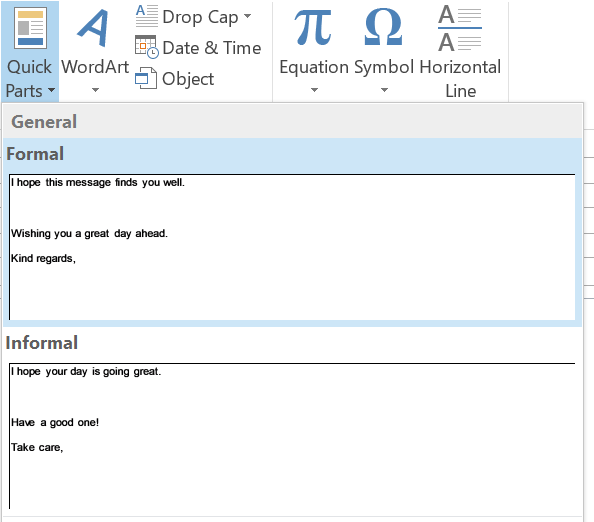
\includegraphics[width=\linewidth]{img/Quick_parts.png}
	\caption{Esimerkkejä Outlookin viestipohjista (Quick parts)}
	\label{fig:Quick_parts}
\end{figure}

\medskip

Lisää Outlookin pikanäppäimiä: \url{https://support.office.com/en-us/article/keyboard-shortcuts-for-outlook-3cdeb221-7ae5-4c1d-8c1d-9e63216c1efd}

\subsection{Youtube}

Aika usein on katsottava esitys tai luento tai opeteltava jonkin ohjelman käyttöä Youtubesta. Nopeuttamalla tunnin videota esimerkisksi 1.5-kertaiseksi säästät jo 20 minuuttia! Melkeinpä mitä tahansa videota voi nopeuttaa 1.25 kertaiseksi ja hitaita puhujia voi olla jopa miellyttävämpää kuunnella tuplanopeudella.

\keys{\shift + .} Nopeuta videota

\keys{\shift + ,} Hidasta videota

\keys{F} Koko ruudun tila

\keys{\keys{\arrowkeyright}} tai \keys{L} Mene 5/10 sekuntia eteenpäin

\keys{\keys{\arrowkeyleft}} tai \keys{J} Mene 5/10 sekuntia taaksepäin

\url{https://youtu.be/UlB7TJ6cTx4}

\medskip

Myös monissa muissa videopalveluissa on vastaavanlaisia toiminnallisuuksia.

\subsection{Suurennuslasi}

Oletko koskaan tihrustanut teams-esitystä pieneltä läppärin ruudulta? Zoomaaminen tekee seuraamisesta usein huomattavasti miellytävämpää. (ks. myös teamsin sisäänrakennetut "Focus" \& "Fullscreen" -toiminnot.)

\keys{Win} + \menu{+} suurentaa

\keys{Win}+\keys{-} pienentää

\keys{Win}+\keys{Esc} sulkee suurennuslasin

\keys{Win}+\keys{\shift}+\keys{m} avaa asetukset, jossa esim. zoomauksen väliä (zoom increment) voi olla hyvä säätää. Esim. 10\% toimii aika mukavasti.

\subsection{Tumma tausta}

Ehkä hieman yllättävä tapa tehokkuuteen on tumman taustan vaihtaminen. Silmät eivät väsy lukiessa ja tietokoneen käyttäminen on pienen totuttelun jälkeen yllättävän paljon miellyttävämpää. Tässä muutama oleellisin, nykyään melkein minkä tahansa ohjelman saa tummalla teemalla.

\subsubsection{Windows}
Paina \keys{Win} + \keys{Kirjoita "tumma teema" tai "dark theme"} + \keys{\return} ja vaihda teema tummaksi. Saatat joutua vaihtamaan alta vielä korostusväriä. Tumma teema tulee tämän jälkeen automaattisesti moneen muuhun ohjelmaan.

\subsubsection{Microsoftin ohjelmat}

Mikäli tummuus ei siirry suoraan Microsoftin ohjelmiin, saa asetukset vaihdettua myös itse.

\menu{Tiedosto > Tili > Officen Teema > Musta}

\menu{File > Account > Office Theme > Black}

\begin{figure}[H]
	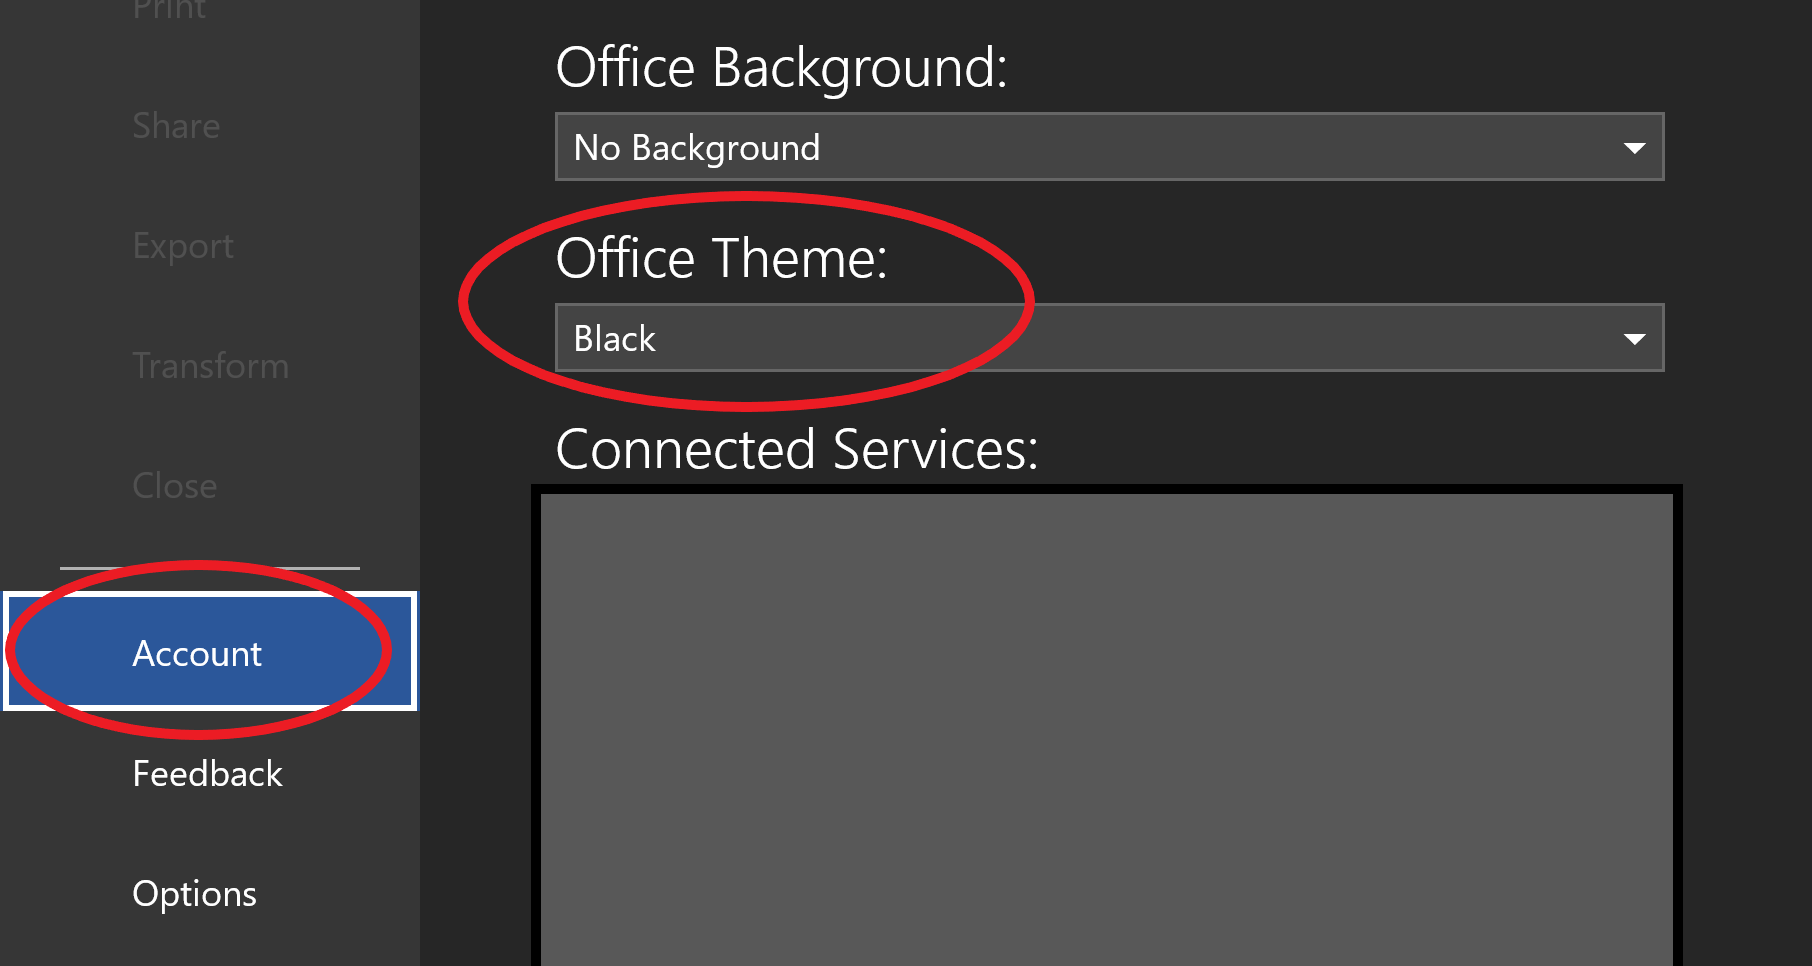
\includegraphics[width=\textwidth]{img/Dark_theme_word}
\end{figure}

\textbf{HUOM!} Wordissä tekstin ja taustan värit saa käännettyä valitsemalla 

\menu{Näytä > Vaihda tiloja}

\menu{View > Switch Modes}

\begin{figure}[H]
	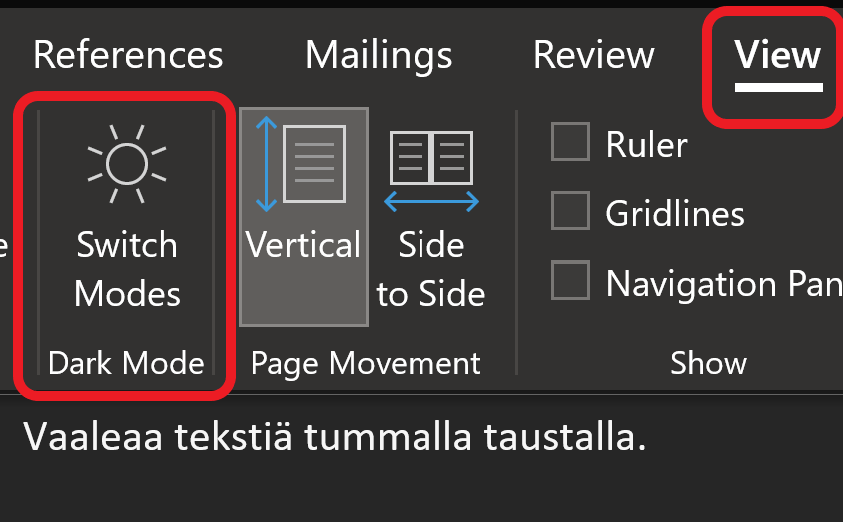
\includegraphics[width=0.5\textwidth]{img/dark_word}
\end{figure}

\subsubsection{Adobe Reader}

Yleensä pitkiä tekstejä luetaan kuitenkin PDF-tiedostoista. Siinä tekstin ja taustan värit saa määriteltyä haluamakseen.

\begin{enumerate}
	\item \keys{Ctrl}+\keys{k} avaa asetukset 
	\item \menu{Esteettömyys > Korvaa asiakirjan värit > Valitse värimalli}
	\item \menu{Accessibility > Replace Document Colors > Custom Color}
	\item Tumman harmaa tausta ja vaalean harmaa teksti ovat miellyttävämpiä silmille kuin täysin musta ja valkoinen.\footnote{esim. RGB (36,36,36) ja (241,241,241)}
\end{enumerate}

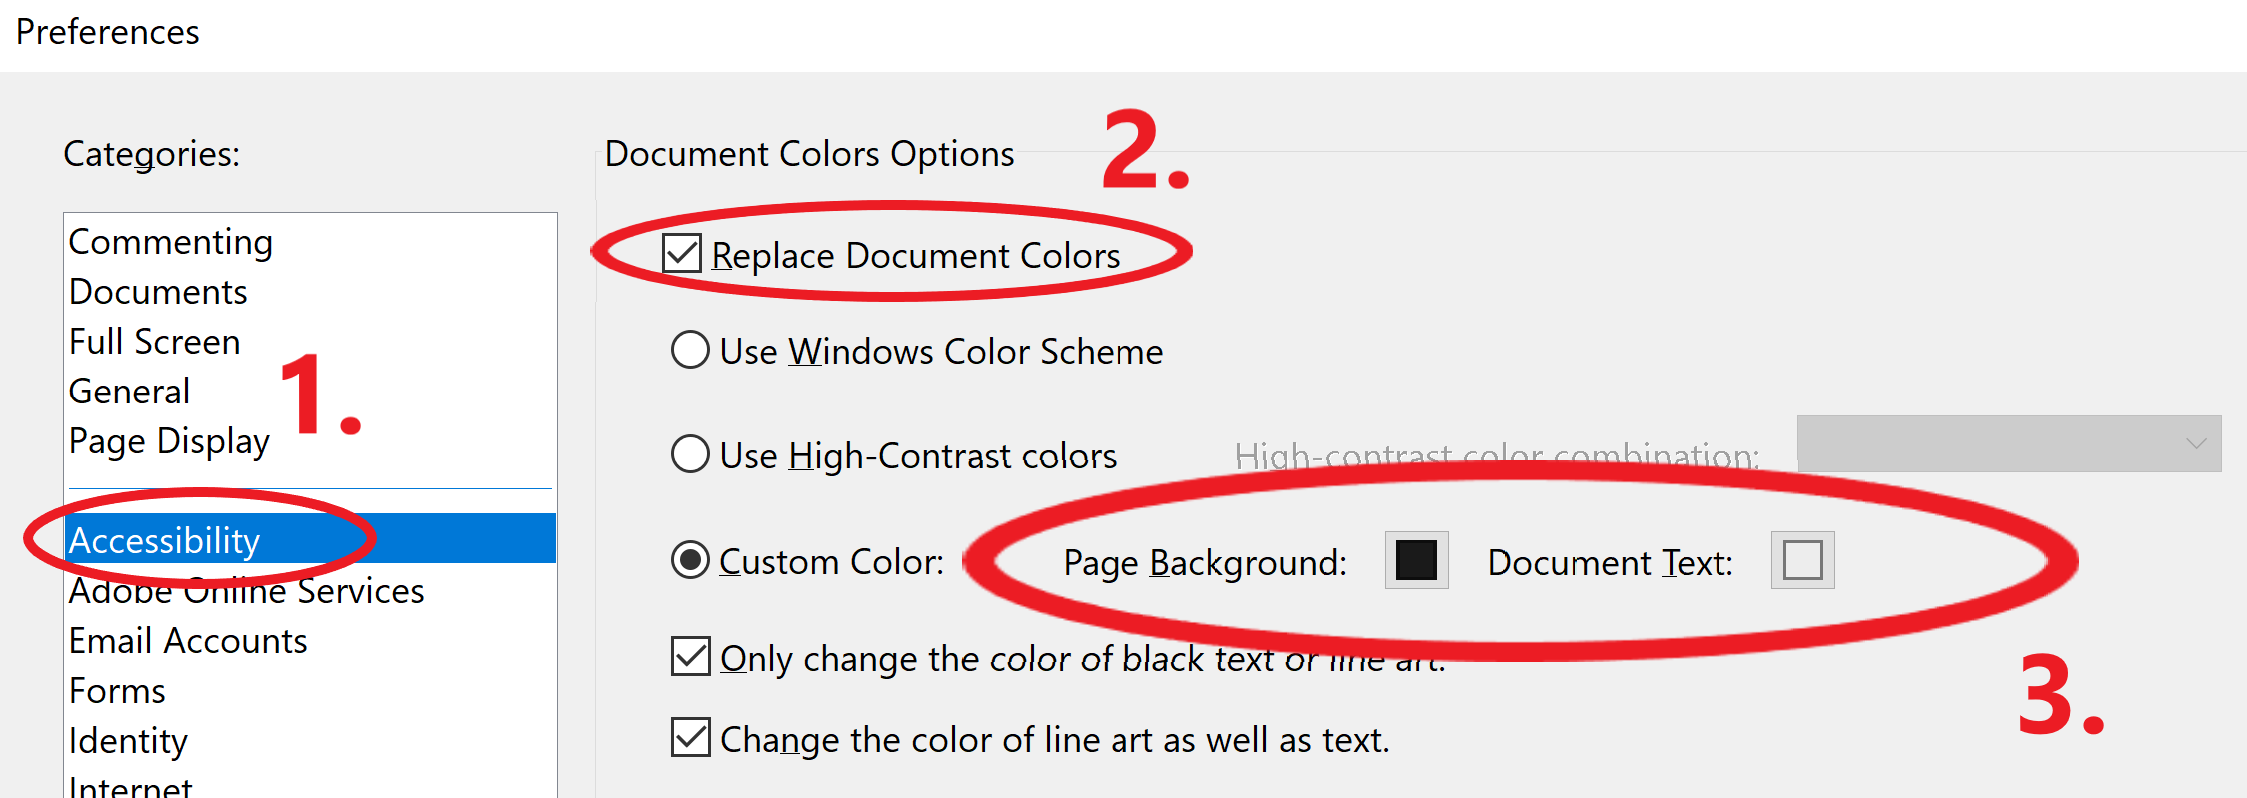
\includegraphics[width=\textwidth]{img/adobe_reader}

Jatkossa tumman ja vaalean taustan välillä voi vaihdella kätevästi vain painamalla \keys{Ctrl}+\keys{k}  ja klikkaamalla sivun ylälaidasta \menu{Korvaa asiakirjan väri} tai \menu{Replace Document Colors}

\pagebreak \section{Ladattavat ohjelmat ja koodi}
Osiota \fullref{perus} lukuunottamatta tarvitset seuraavat ohjelmat ja koodin.





\subsection{Zotero}
\url{https://www.zotero.org/download/}


Lataa sekä ''Zotero for Windows'', että ''Zotero Connector''. 

\subsection{Autohotkey}
\url{https://www.autohotkey.com/download/}
Valitse ''Download Autohotkey Installer''

\subsubsection{Autohotkey scriptit} \label{downloads}

\begin{framed}
	
	\underline{1.Mene osoitteeseen:}
	
	\url{https://github.com/samuelsaari/workflow})
	
	\medskip
	
	\underline{2. Lataa tiedostot}
	
	windows\_workflow.ahk
	
	stata\_workflow.ahk
	
	word\_macros.txt
	
	\medskip
	
	\underline{3.Lataa myös tiedostot kansiosta Useful\_material}
	
	
	%% Erityisesti \textbf{shorcut\_chart.pdf} on hyvä katsoa läpi, koska siinä näkyy suhteellisen havainnollisesti suurin osa autohotkey-pikanäppäimistä. Muita tiedostoja Useful\_material-kansiosta et välttämättä tarvitse akuutisti, mutta niille tulee luultavasti käyttöä jossain vaiheessa, joten ne on hyvä ladata valmiiksi.
	
\end{framed}


\medskip

Ahk-scriptit aktivoituvat tuplaklikkaamalla. Jotta scripti pyörii myös sen jälkeen, kun olet käynnistänyt tietokoneen uudestaan, luo tiedostosta pikakuvake ja laita se windowsin käynnistys-kansioon.

\medskip

\emph{WINDOWS 10}: Paina \keys{Win}+\keys{r} ja kirjoita ilmestyvään ruutuun \mybox{shell::startup} ja paina \keys{\return}. Tämän jälkeen Copy-pastaa luomasi pikakuvake aloituskansioon

\medskip

%\emph{WINDOWS 7}: Paina \keys{Win}+\keys{r} ja kirjoita ilmestyvään ruutuun 

%\emph{C:/users/\textbf{*YOURUSERNAME*}/AppData/Roaming/Microsoft/Windows/Start Menu/Programs/Startup} 

%ja paina \keys{\return}. *YOUR USERNAME* korvataan siis sinun käyttäjätunnuksellasi, esim. mmak (sama millä kirjaudutaan windowsiin ja Outlook webiin)
%Tämän jälkeen Copy-pastaa luomasi pikakuvake aloituskansioon.


\subsection{Word}
Tarvitset koodinpätkän, jotta seuraavat jutut toimivat. Kun word on auki paina \keys{Alt}+\keys{F11} ja Copy-pastaa (\keys{Ctrl}+\keys{c} \& \keys{Ctrl}+\keys{v}) tiedostossa \textbf{word\_macros.txt} oleva koodi käytettävissä olevaan isoon tilaan. Tiedosto löytyy \href{https://github.com/samuelsaari/workflow}{Githubista}, ks. osio \ref{downloads}. Tallenna macrot (\keys{Ctrl}+\keys{s}) ja palaa Wordin perunäkymään.

Tämän jälkeen on vielä alustettava pikanäppäimet ennen ensimmäistä käyttöä:

\menu{Näytä > Makrot > Näytä makrot} 

\menu{View > Macros > View Macros} ja aja "A\_RUN\_SHORTCUTS" -makro.

Jos pikanäppäimet eivät toimi, käynnistä word uudelleen. 

%\begin{lstlisting}[frame=single]
%\end{lstlisting}


\section{Autohotkey pikanäppäimet Windosille ja Statalle}
Pikanäppäimet löytyvät \*.ahk kooditiedostoista, jotka olet ladannut linkin \url{https://github.com/samuelsaari/workflow} takaa (ks. osio \ref{downloads}).

\subsection{Ohjelmien käynnistäminen ja niiden välillä liikkuminen}\label{roar}

Suurin osa pikanäppäimistä avaa/aktivoi ohjelman tai ikkunan, mutta myös joitain usein toistuvia toimia on automatisoitu \footnote{ks. windows\_workflow.ahk tiedosto}.

\medskip

Alla eritelty joitain esimerkkejä pikanäppäimistä.

Yleisesti \keys{Alt}+\keys{"näppäin"} tekee kullekin ohjelmalle jotain seuraavista:

- Jos ohjelma ei ole auki, avaa ohjelma

- Jos ohjelmasta on yksi ikkuna auki, ikkuna minimoidaan

- Jos ohjelmasta on yksi ikkuna käynnissä, mutta ei näy näytöllä, se saadaan näkyviin

- Jos ohjelmasta on useampi ikkuna käynnissä, pikanäppäin kierrättää näitä ikkunoita

\medskip

\keys{Alt}+\keys{1} Stata

\keys{Alt}+\keys{2} Outlook

\keys{Alt}+\keys{3} Adobe Reader

\keys{Alt}+\keys{§} PowerPoint

\keys{Alt}+\keys{W} Word

\keys{Alt}+\keys{Q} Excel

\keys{Alt}+\keys{E} Zotero

\keys{Alt}+\keys{CapsLock} Firefox

\keys{Alt}+\keys{\shift} Chrome

\keys{Alt}+\keys{A} Kansiot

\keys{Alt}+\keys{D} Teams

\keys{Alt}+\keys{Z} Zoom

\keys{Alt}+\keys{B} (Bluetooth-)asetukset

\keys{Alt}+\keys{N} Notepad

\keys{Alt}+\keys{Ctrl} Spotify

\keys{Alt}+\keys{Esc} Sulje käynnissä oleva ohjelma

\textbf{Protip:} Katso kaikki komennot tai muokkaa pikanäppäimiä tiedoston \emph{windows\_workflow.ahk} kautta. Jos haluat lisätä uusia ohjelmia, kannattaa tallentaa \emph{tooltip.ahk} sopivaan sijaintiin, jonka jälkeen voit voit tarkastella tarvittavia parametrejä \keys{Ctrl}+\keys{pitkä} näppäinyhdistelmällä. Yksityiskohdat tiedoston \emph{windows\_workflow.ahk} kohdasta \emph{Toggle tooltip}.

\subsection{Viitteet}

\subsubsection{Viitteiden lisääminen Zoteroon Firefoxissa ja Chromessa}
\keys{\ctrl + \shift + S}

Tämä toimii jossain määrin myös ilman Autohotkeytä, mutta tällä lailla viitteet tallentuvat pdf-tiedostoineen varmemmin.

Firefoxin ja Zoteron connectorin pikanäppäimet menevät päällekäin, joten Chrome voi olla alkuun kätevämpi. Jos haluat käytttä firefoxia sisäänrakennetun pikanäppäimen saa poistettua seuraavasti:
\begin{itemize}
	\item Kirjoita \emph{about:addons} osoiteriville (Esim. \keys{Ctrl}+\keys{K})
	\item Valitse rattaan kuva oikeasta yläreunasta ja sieltä \menu{Manage Extension Shortcuts}
\end{itemize} 

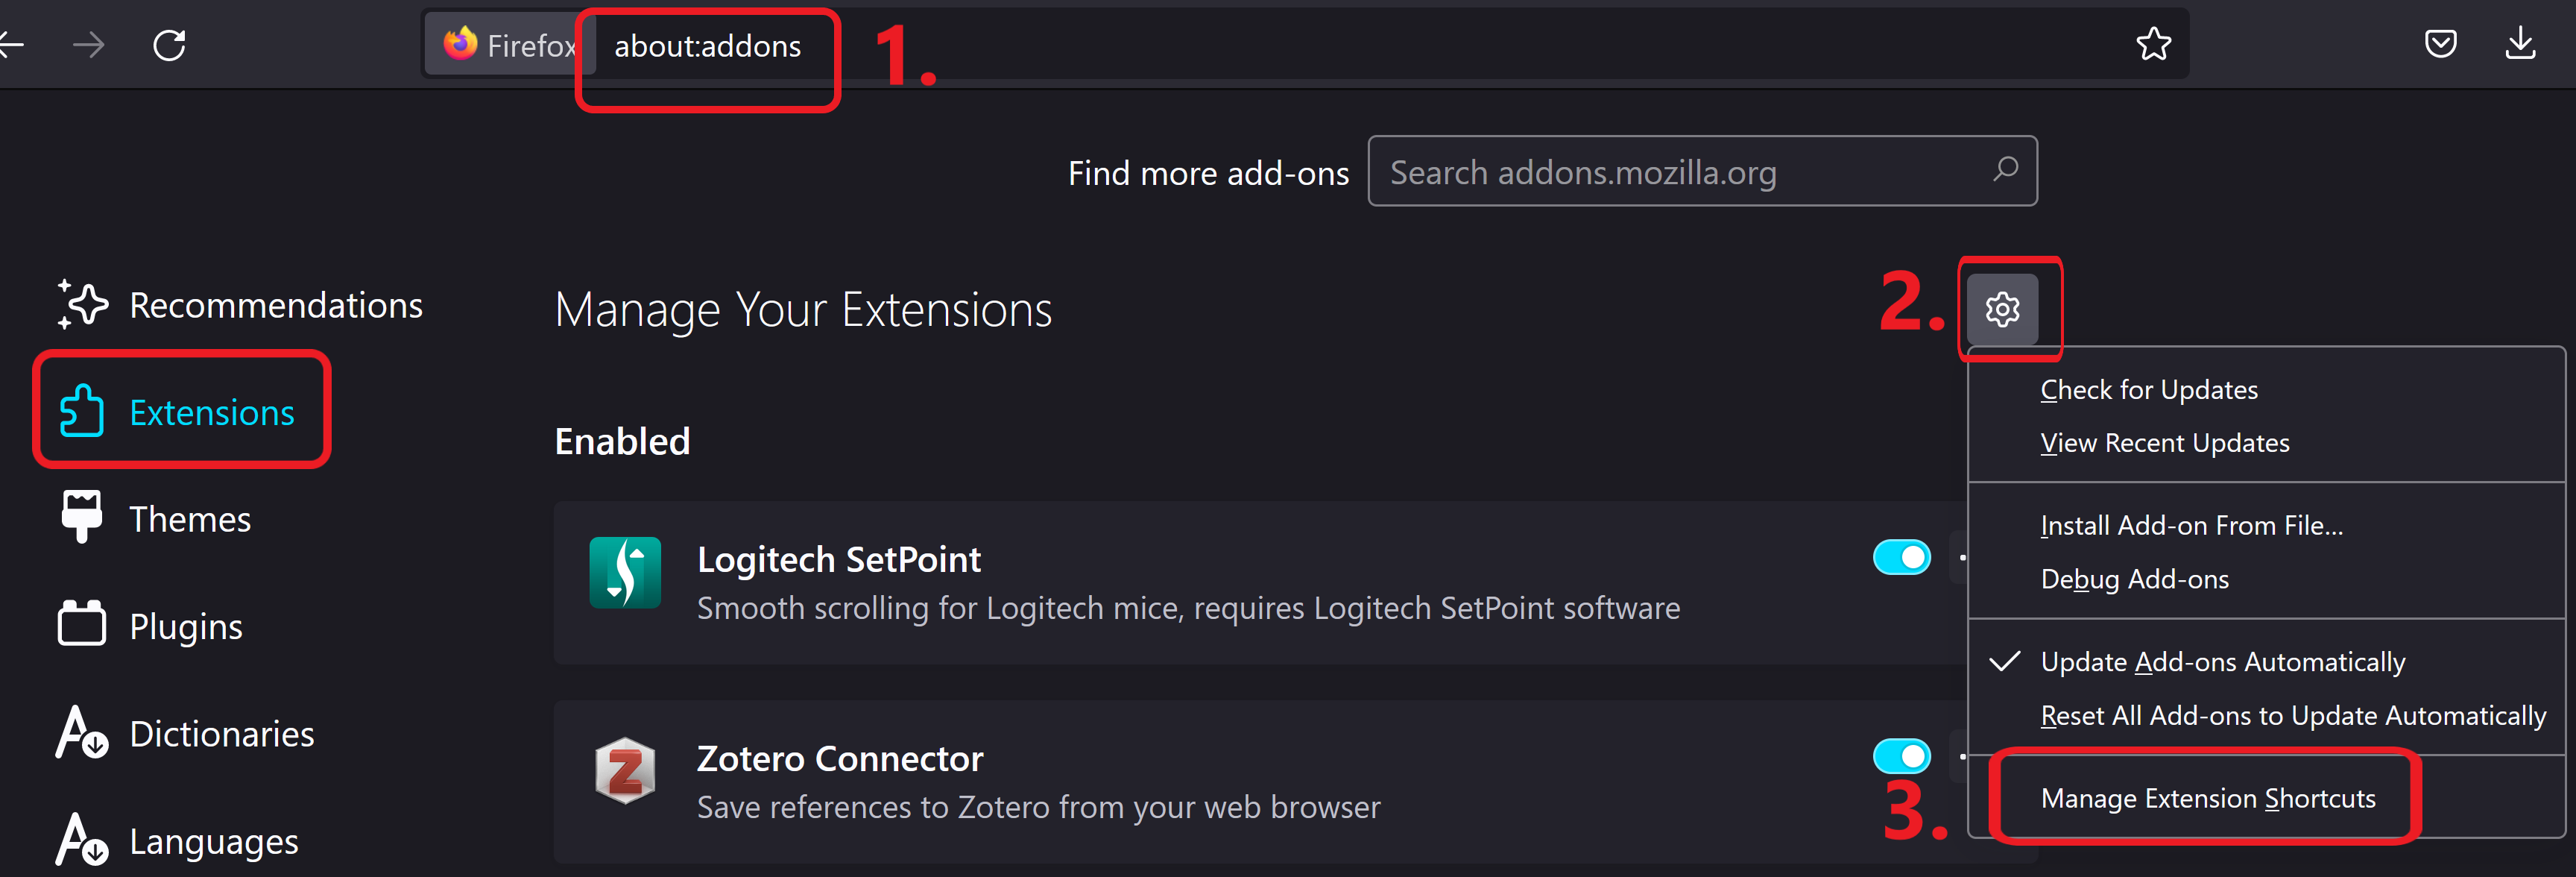
\includegraphics[width=\textwidth]{img/firefox1}
\begin{itemize}
	\item Poista firefoxin pikanäppäin painamalla roskiksen kuvaa
\end{itemize}
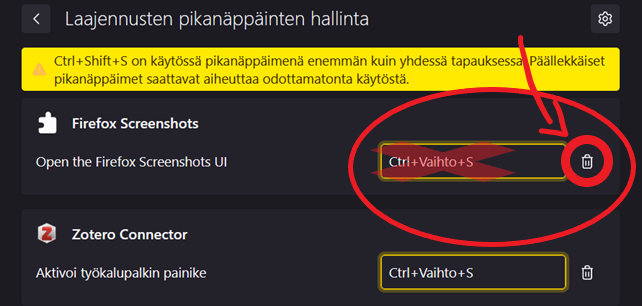
\includegraphics[width=\textwidth]{img/firefox2}

\subsubsection{Lähdeviittaaminen Wordissa}

\keys{\ctrl + å}
Tämä pikakomento tekee monta asiaa, riippuen tilanteesta:

- lisää uuden viitteen

- muokkaa olemassa olevaa viitettä

- poistaa kirjoittajan (2019) viittauksesta

- Palauttaa kirjoittajan viitteeseen (Saari, 2019). Siis edellisen käänteistoiminto

- avaa viittausikkunan, jos se on olemassa, mutta ei ole aktiivinen


Lisäksi on hyvä tietää, että kaksoispisteen \keys{:} avulla viitteen perään saa sivunumerot.

Kun dokumentti on valmis, lisää lähdeluettelo wordiin pikanäppäimellä:

\keys{\ctrl}+\keys{Alt}+\keys{B}

Olemassa olevan lähdeluettelon päivitys:

\keys{\ctrl + \shift+ å}

Näin välttyy kokonaan viitteiden tarkistamiselta, ja monelta muulta harmilta.

\subsubsection{Lähdeviitteiden tarkistaminen Wordissa (extra)}
Mikäli et ole käyttänyt Zoteroa tai olet poistanut Zotero-linkityksen, käytettyjen lähdeviitteiden tarkistaminen onnistuu kätevästi jakamalla ruutu kahtia.

\menu{Näytä > (Järjestä) > Jaa }

\menu{View > (Arrange) > New Window}

Ks. lisätiedot:

\url{https://support.office.com/en-us/article/view-two-parts-of-a-document-at-the-same-time-in-word-for-mac-1adf3317-0ec4-4568-ad32-6f68b3e4b386}

Tämän jälkeen lue teksti alusta loppuun ja merkitse käytetyt viitteet värittämällä ne. Yhden lähdeviitteen (kappaleen) korostaminen onnistuu pikakomennolla

\keys{Ctrl}+\keys{ö}. 

Jos haluat poistaa värityksen yhdestä viitteestä (kappaleesta) paina

\keys{ctrl}+\keys{ä}

Kun olet päässyt tekstin loppuun, voit poistaa värjäämättömät viitteet, poistaa värit ja dokumentin kahtia jaon. Jos käytät Zoteroa niin tällaista tarkistustahan ei tarvi tehdä!

\subsection{Stata}

Alla muutama esimerkki. Loput pikakomennot ja niiden muokkaus \emph{stata\_workflow.ahk} tiedoston kautta.

\medskip

\keys{Alt}+\keys{1} Käynnistää Statan ja pyörittää kaikkia auki olevia ikkunoita (ks. \ref{roar})

\keys{Win}+\keys{1} Jos olet kiinnittänyt Statan ensimmäiseksi työkalupalkkiin, tekee saman kuin edellinen, mutta voit seurata missä kohtaa menet. Suositeltavaa, sillä muut vastaavat pikanäppäimet alkavat Windows-napilla.

\keys{Win}+\keys{CapsLock} Stata pääikkuna

\keys{Win}+\keys{\shift} Do-file

\keys{Win}+\keys{\textgreater} Ensin Statan pääikkuna, Sitten do-file

\keys{Win}+\keys{Q} Editor

\keys{Win}+\keys{A} Graph

\keys{Win}+\keys{Z} Viewer

\medskip

\keys{\ctrl}+\keys{D} Aja koko do-file

\keys{\ctrl + \return} Aja rivi koodia

\keys{Alt}+\keys{\return} Aja koodia merkkien \keys{\{} \keys{\}} välissä

\keys{Ctrl}+\keys{Alt}+\keys{B} Aja do-file siihen asti, missä tekstikursori on (kätevä, mutta ei toimi 100\% luotettavasti)


%   \section{Extra}
%    You can visualize paths \directory{/home/moose/Desktop/manual.tex}
%    or menus \menu{View > Highlight Mode > Markup > LaTeX} or key
%    press combinations: \keys{\ctrl + \shift + F} is for formatting
%    in Eclipse.
%    You can also visualize \keys{\tab}, \keys{\capslock}, \keys{\Space}, 
%    \keys{\arrowkeyup} and many more.
%    Let's try some more: \keys{a}, \keys{ä} 


\end{document}